\documentclass[letterpaper, twocolumn]{article}

\usepackage{lipsum}
\usepackage{mathptmx}
\usepackage[usenames,dvipsnames]{xcolor}
\usepackage{graphicx}
\usepackage{tikz}
\usetikzlibrary{arrows}
\usetikzlibrary{arrows.meta}

\author{James~T.~Murphy~III\thanks{\texttt{jamesmurphy@math.utexas.edu}}\and{}Skyler~Thomas\thanks{\texttt{skylerthomas0@gmail.com}}}

\title{Learning Breakout using NEAT}

\begin{document}
\maketitle{}
\begin{abstract}
    We present a replication of the learning of a version of
    Breakout via machine learning, specifically using an evolutionary algorithm known as NEAT.
    We show that given the current and past few game states as inputs, NEAT
    can evolve a neural network that can completely clear a game of Breakout,
    and we identify three eras of learning that occur during training.
\end{abstract}

\section{Introduction}

Recent advances in machine learning have spurred both research interest in and popular applications
of neural networks.
A popular application of particular interest is teaching neural networks to play video games.
Such games often involve complex and potentially long-term strategies to play optimally.
It was demonstrated in~\cite{mnih2013playing} and~\cite{mnih2015human} that deep reinforcement learning can be used to train a neural network
to play a wide array of Atari games.
Similarly, YouTuber SethBling demonstrated that a neural network could learn via evolution to play the Super Nintendo game Super Mario World~\cite{sethbling2015}.
We took inspiration from these projects and have used the same evolutionary algorithm to train a neural network
to play a version of the Atari game Breakout.

\begin{figure}[ht!]
    \centering
    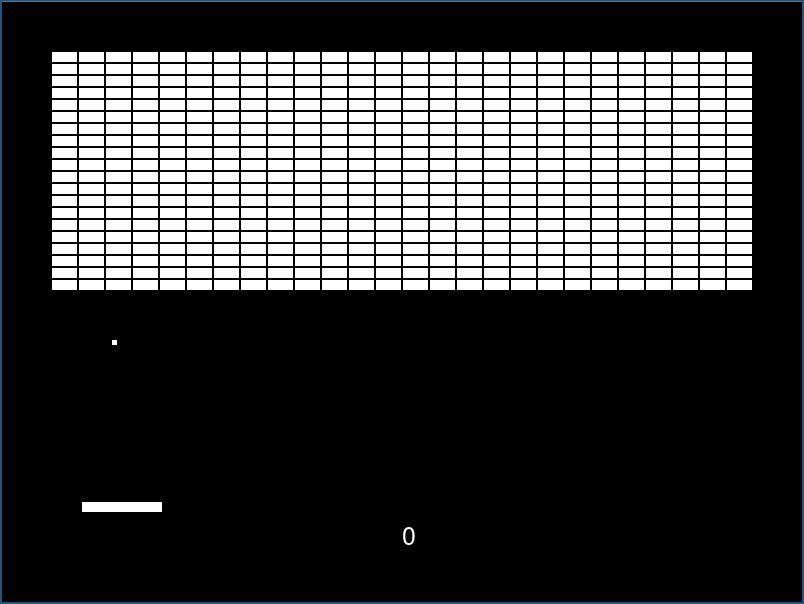
\includegraphics[width=.45\textwidth]{breakout.png}
    \caption{The version of Breakout we used.}
\end{figure}

Breakout is a game where the user moves a paddle at a fixed distance
from the bottom of the screen in an attempt to destroy as many blocks as possible
by bouncing a ball off the paddle.
For each block that is hit, a point is awarded.
This continues until either the player misses the ball or all 520 blocks are hit.

The evolutionary algorithm we employ is NeuroEvolution of Augmenting Topologies
(NEAT)~\cite{stanley2002evolving, stanley2002efficient}.
NEAT is a type of genetic algorithm that follows biological meta-heuristics.
In NEAT, neural network nodes and weights are modeled as genes.
Genomes are randomly mutated by adding/deleting nodes, adding/deleting connections, changing connection weights, etc.
After mutation, individuals are ranked by their fitness at performing a certain task, in our case playing a game of Breakout.
The best performing individuals are allowed to mate using a genetic crossover algorithm,
producing children that compose the next generation of individuals.
Crossover is made possible by keeping track of different species that develop and
only allowing mating within the same species.
This process is repeated until some fitness threshold is reached, typically
that the most fit individual succeeds at a particular task, in our case achieving a maximum score in Breakout.

\section{Results}
We find there are qualitatively three eras of evolution of the population of
networks:
\begin{enumerate}
    \item{}\emph{Pre-ball-tracking era}: a network typically does nothing or makes a few small adjustments at the very beginning of the game, scoring a minimal number of points usually $0$ to $30$.
    \item{}\emph{Ball-tracking era}: a network definitively makes an effort to keep the paddle horizontally aligned with the ball. 
	    It clears a sizeable portion of the blocks, and only fails in edge cases or by infinitely looping without clearing some remaining blocks. 
		It typically scores $100$ to $400$ points.
    \item{}\emph{Aiming era}: a network tracks the ball as before, but also makes sporadic adjustments to aim at remaining blocks. 
	    It clears all or nearly all of the blocks, achieving a score from
		$500$ to the maximum $520$.
\end{enumerate}
A large percentage of the time, around $90\%$ of attempts, the NEAT algorithm stagnates at a local maximum
fitness somewhere in the first two eras.
Simply repeating the experiment a sufficient number of times eventually yields a trained network that
can achieve the maximum score.
The resultant network is typically very small, having 5 or less non-input nodes and under 15 total connections.
\begin{figure}[ht!]
    \centering
    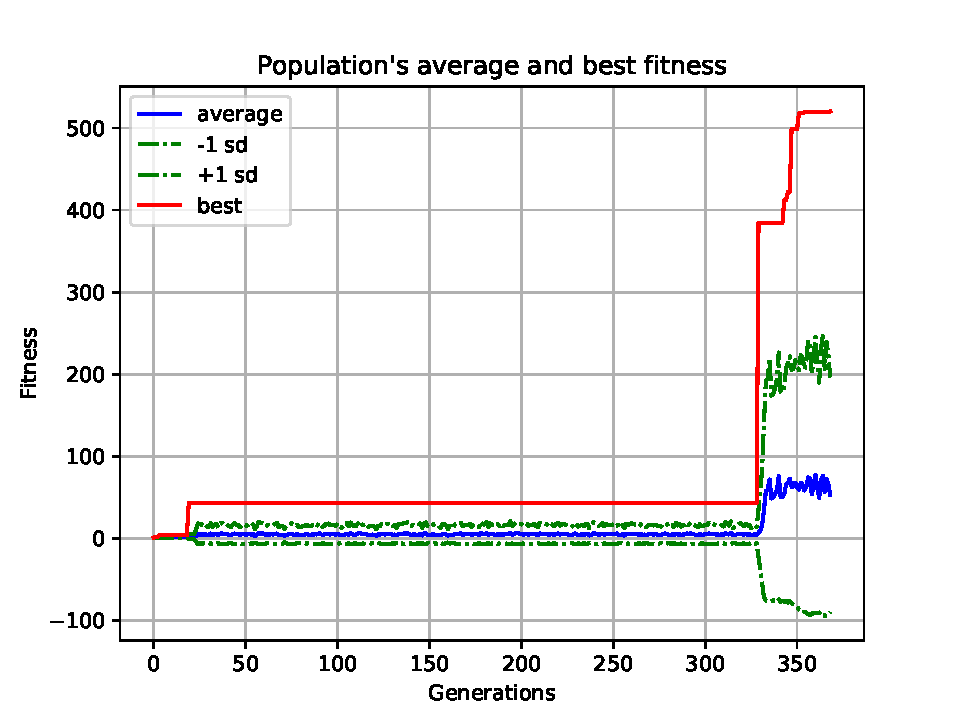
\includegraphics[width=.54 \textwidth]{avg_fitness.pdf}
    \caption{A successful training experiment. In this case, the pre-ball-tracking era lasts
        until around generation 325, when a network abruptly learns how to track the ball.
        The ball-tracking era then lasts until around generation 350, when a
	network learns to avoid missing stray blocks. 
	The aiming era is reached in the last few generations.
        Generations, each of 200 individuals, took an average time of 2.835 seconds to evaluate running on an
        Intel Core i7-4790K @ 4.00GHz in parallel on 6 cores. The total runtime was around 17.5 minutes.}
\end{figure}

It turned out to be critical to the success of the NEAT algorithm that several previous game states (3 is sufficient) were included as inputs to the neural networks.
Giving only the current state, including the direction of the ball, as input was not sufficient in any
of our experiments to produce a network that could even reliably track the ball.

Also, it was necessary to train the network with a fixed initial condition (initial ball speed and angle).
We found that randomizing the initial condition made it too hard for evolution to select for individuals
that could track the ball because, for instance,
a network that pressed no buttons at all could earn sometimes 50 points with a very lucky initial condition.
Although the initial condition ultimately used was deterministic,
the final trained networks do not simply memorize a sequence of inputs that work for the initial condition.
Indeed, the final networks turn out to be far too small for such memorization to be possible.
Further, testing the most fit network with new initial conditions proved that its performance does generalize.

Another pitfall that was avoided was giving too many inputs to the networks.
If the game state fed to the network
included information about all 520 blocks, then regardless of whether the game history was given,
none of our experiments produced a network that could reliably track the ball.
The vast majority of networks trained in this manner did precisely nothing, making no button presses
at all.
On the other hand, training was able to produce an aiming era individual
when the density of blocks remaining in a few predetermined regions were passed as inputs.
Training also succeeded when the game state passed to the networks included no information about the remaining blocks whatsoever, i.e.\ a network that saw only the paddle and ball could still achieve a maximum score.

\def\layersep{2.0cm}
\begin{figure}[ht!]
	\centering
	\begin{tikzpicture}[shorten >=1pt,->,draw=black!50, node distance=\layersep]
		\tikzstyle{every pin edge}=[<-,shorten <=1pt]
		\tikzstyle{neuron}=[circle,fill=black!25,minimum size=17pt,inner
		sep=0pt, color=darkgray]
		\tikzstyle{negconn}=[color=BurntOrange]
		\tikzstyle{posconn}=[color=CornflowerBlue]

		\node[neuron, pin=left:{\small$paddle[3].x(t)$}] (I-2) at (0,-1) {};
		\node[neuron, pin=left:{\small$paddle[2].x(t-3)$}] (I-4) at (0,-2) {};
		\node[neuron, pin=left:{\small$paddle[2].x(t-1)$}] (I-5) at (0,-3) {};
		\node[neuron, pin=left:{\small$paddle[2].x(t)$}] (I-3) at (0,-4) {};
		\node[neuron, pin=left:{\small$ball.x(t-3)$}] (I-6) at (0,-5) {};
		\node[neuron, pin=left:{\small$ball.x(t-2)$}] (I-1) at (0,-6) {};
		\node[neuron, pin=left:{\small$ball.x(t-1)$}] (I-7) at (0,-7) {};
		\node[neuron, pin=left:{\small$ball.y(t-3)$}] (I-8) at (0,-8) {};
		\node[neuron, pin=left:{\small$paddle[0].x(t)$}] (I-9) at (0,-9) {};

		\node[neuron,pin={[pin edge={->}]right:L}, right of=I-3] (L) {};
		\node[neuron,pin={[pin edge={->}]right:R}, right of=I-8] (R) {};

		\draw[negconn, line width=.95mm] (I-1) -- (L);
		\draw[posconn, line width=.32mm] (I-2) -- (L);
		\draw[posconn, line width=.42mm] (I-3) -- (L);
		\draw[posconn, line width=.87mm] (I-4) -- (L);
		\draw[negconn, line width=.14mm] (I-5) -- (L);
		\draw[negconn, line width=.78mm] (I-6) -- (L);
		\draw[posconn, line width=.16mm] (I-7) -- (L);

		\draw[posconn, line width=.37mm] (I-7) -- (R);
		\draw[posconn, line width=.41mm] (I-8) -- (R);
		\draw[negconn, line width=.38mm] (I-9) -- (R);
	\end{tikzpicture}
	\caption{The most fit genome in one experiment with the network blind
	to the remaining blocks. Notice how it approximately hits left if the
	ball is left of the paddle, and it approximately hits right if the
	ball is right of the paddle. See the methods section for an explanation
	of the variables.}
\end{figure}

\section{Methods}

The source code and configuration of our experiments are publicly available
at~\cite{neatbreakout}.

We modified a Pygame implementation (cf.~\cite{pygame}) of Breakout (cf.~\cite{max00355breakout}) to allow
human mouse input and human keyboard input (for testing purposes), or automated keyboard input.
Then we used NEAT-Python (cf.~\cite{neatpython}) to run the NEAT algorithm.

To allow the neural network to play Breakout,
each frame a representation of the game state is computed and
passed as the input layer to a neural network.
The neural network has two outputs ``L'' and ``R'', which are binarized
and taken to indicate whether the left or right arrows are being pressed by the neural network.

The representation of the game state includes the following information:
\begin{itemize}
    \item{} $ball.x$, $ball.y$: the $x$ and $y$ coordinates of the ball,
	    normalized as a percentage of the width of the game,
    \item{} $ball.xdir$, $ball.ydir$: the $x$-direction $\pm1$ and $y$-direction $\pm 1$ of the ball,
    \item{} $ball.angle$: the angle of the ball, normalized as a percentage of
	    $2\pi$,
    \item{} $paddle[0].x$, $paddle[1].x$, $paddle[2].x$, $paddle[3].x$: the $x$
	    coordinates of the left endpoints of each of the sections of
		the paddle, normalized as a percentage of the width of the
		game,
    \item{} the history of the previous four up to a fixed number of time steps
	    in the past,
    \item{} (optionally) the density of remaining blocks in e.g.\ each of the four block quadrants or similar fixed configuration of predetermined regions of blocks.
\end{itemize}

After carefully choosing the parameters of the algorithm, a neural network
is trained to play Breakout using NEAT with the final score of playing a game
being the fitness function.
Success of the training is \emph{very} sensitive to changes in hyperparameters
of NEAT, so the interested reader should view the sample training configuration
file in~\cite{neatbreakout}.

\section{Discussions}

Although NEAT did eventually produce neural networks that can achieve the maximum score
in Breakout, NEAT was very prone to stagnation at a local maximum fitness.
We suspect that this was mainly due to the nature of how training was setup.
Fitness was evaluated by allowing a network to play a whole game of Breakout start to finish.
This means that small changes in the network could result in drastically different scores, making it hard
to make the kind of incremental progress that evolution can select for easily.
We suggest that anyone interested in repeating this experiment make the following changes to
the training setup:
\begin{enumerate}
    \item{} Generate initial board setup, paddle location, ball location, speed, and direction randomly.
    \item{} Make the fitness of an individual the score that the network receives in 5 seconds of simulated gameplay, averaged over 10 trials.
    \item{} Optionally, change the scoring mechanism to assign $\gamma^n$ points for a block destroyed
        at frame $n$ in training, where $\gamma<1$ is very close to $1$. 
        This encourages networks not only to destroy the blocks, but to do so as quickly as possible.
\end{enumerate}

We suggest the previous changes in order to make it easier for evolution to select for incremental progress.
Indeed, in both~\cite{mnih2013playing} and~\cite{mnih2015human} these aspects are already present,
though no evolutionary algorithm is used, and apparently much greater success is achieved there than here.
For Breakout, the changes were not strictly necessary, but originally we attempted to use an analogous
setup to train neural networks to play Tetris.
For Tetris, we had no success, but we believe that it may be possible to learn Tetris using NEAT
once the suggested changes are made.

Future work could make a direct comparison between the performance of the most fit individual trained by
NEAT along with several different methods such as Deep Q-learning or other
evolutionary algorithms besides NEAT.
More work is needed to elucidate what aspects of the learning setup are the most important to allow
long-term strategy to develop. For instance, does evolving the network topology provide any benefit over
choosing a fixed network topology?
In conclusion, we consider the experiment a success, but there are
still many improvements yet to be discovered in order to allow neural networks
to learn more and more complex games.

\begingroup
    %\newpage
    \section{References}
    \renewcommand{\section}[2]{}
    \nocite{*}
    \bibliographystyle{abbrv}
    \begin{raggedright}
    \bibliography{master}
    \end{raggedright}
\endgroup
\end{document}
